\documentclass[12pt]{report}
\usepackage[margin=1in]{geometry}
\usepackage{fancyhdr}
\usepackage{listings}
\usepackage{color}
\usepackage{caption}
\usepackage{subcaption}
\usepackage{textcomp}
\usepackage[pdftex]{graphicx}
\definecolor{listinggray}{gray}{0.9}
\definecolor{lbcolor}{rgb}{0.9,0.9,0.9}
\usepackage{circuitikz}
\usepackage{incgraph}
\usepackage[nomessages]{fp}
\usepackage{sevenseg}
\usepackage{float}
\usetikzlibrary{arrows, decorations.markings}

\newcommand{\x}{0}

\pagestyle{plain}
\lstset{
  tabsize=4,
  rulecolor=,
  language={[x86masm]Assembler},
  basicstyle=\scriptsize\ttfamily,
  upquote=true,
  aboveskip={1.5\baselineskip},
  columns=fixed,
  showstringspaces=false,
  extendedchars=true,
  breaklines=true,
  prebreak = \raisebox{0ex}[0ex][0ex]{\ensuremath{\hookleftarrow}},
  frame=single,
  showtabs=false,
  showspaces=false,
  showstringspaces=false,
  identifierstyle=\ttfamily,
  keywordstyle=\color[rgb]{0,0,1},
  commentstyle=\color[rgb]{0.133,0.545,0.133},
  stringstyle=\color[rgb]{0.627,0.126,0.941},
}

\begin{document}
\renewcommand{\thesection}{A}
\section{Block Diagram of Interfacing Devices}
\subsection{The general block diagram of Interfacing through 8255 PPI}
\begin{figure}[h]
  \begin{center}
    \scalebox{0.8}{
  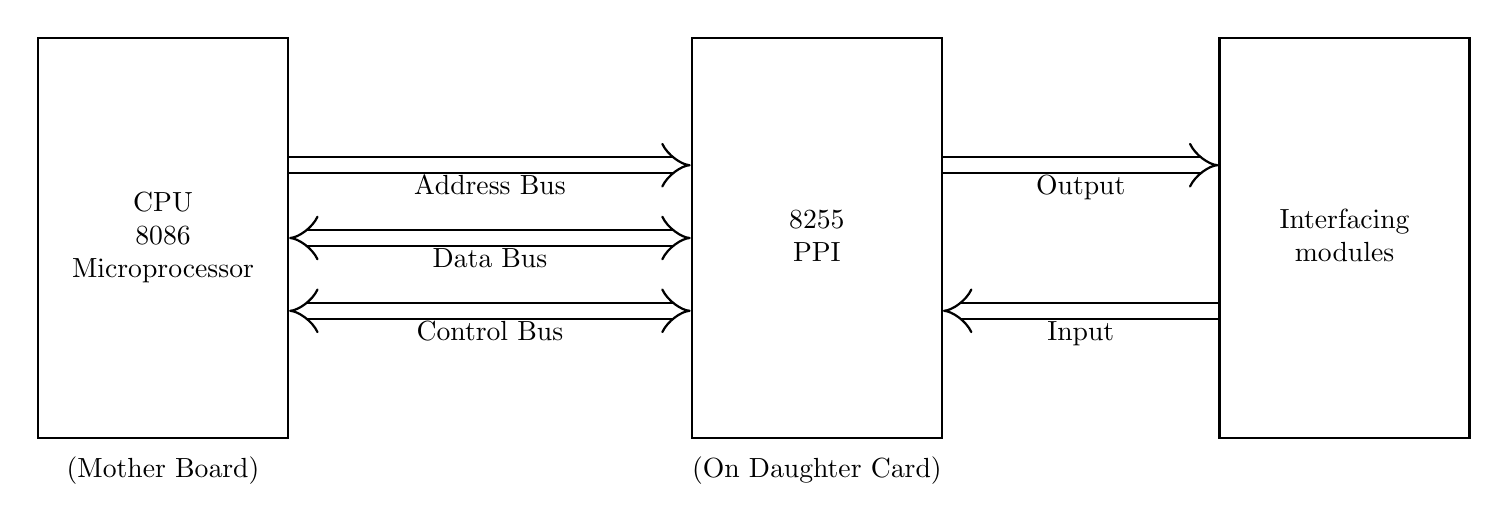
\begin{tikzpicture}[thick, every matrix/.style={ampersand replacement=\&,column sep=3cm,row sep=3pt}]
    \matrix {
      \node[draw,rectangle,minimum height=2in,minimum width=1.25in] (a) {
        \begin{tabular}{c}
          CPU \\ 
          8086 \\
          Microprocessor
        \end{tabular}
      };
      \& 
      \node[draw,rectangle,right of=a,minimum height=2in,minimum width=1.25in] (b) {
        \begin{tabular}{c}
          8255 \\
          PPI
        \end{tabular}
      };
      \& 
      \node[draw,rectangle,right of=b,minimum height=2in,minimum width=1.25in] (c) {
        \begin{tabular}{c}
          Interfacing \\
          modules
        \end{tabular}
      };\\ 
      \node {(Mother Board)} ; \& \node {\hspace{2cm}(On Daughter Card)} ; \& ; \\
    };
    \draw[-implies,double equal sign distance,double distance=5pt] (a.30) -- node[anchor=north]{Address Bus}  (b.150);
    \draw[implies-implies,double equal sign distance,double distance=5pt] (a) -- node[anchor=north]{Data Bus}(b) ;
    \draw[implies-implies,double equal sign distance,double distance=5pt] (a.-30) -- node[anchor=north]{Control Bus}(b.-150) ;
    \draw[-implies,double equal sign distance,double distance=5pt] (b.30) -- node[anchor=north]{Output}(c.150) ;
    \draw[implies-,double equal sign distance,double distance=5pt] (b.-30) -- node[anchor=north]{Input}(c.-150) ;    
  \end{tikzpicture}
}

  \end{center}
\end{figure}

\newpage
\subsection{The control word format of 8255 PPI}
\begin{figure}[h]
  % ~ \scalebox{0.7}{
  \begin{center}
    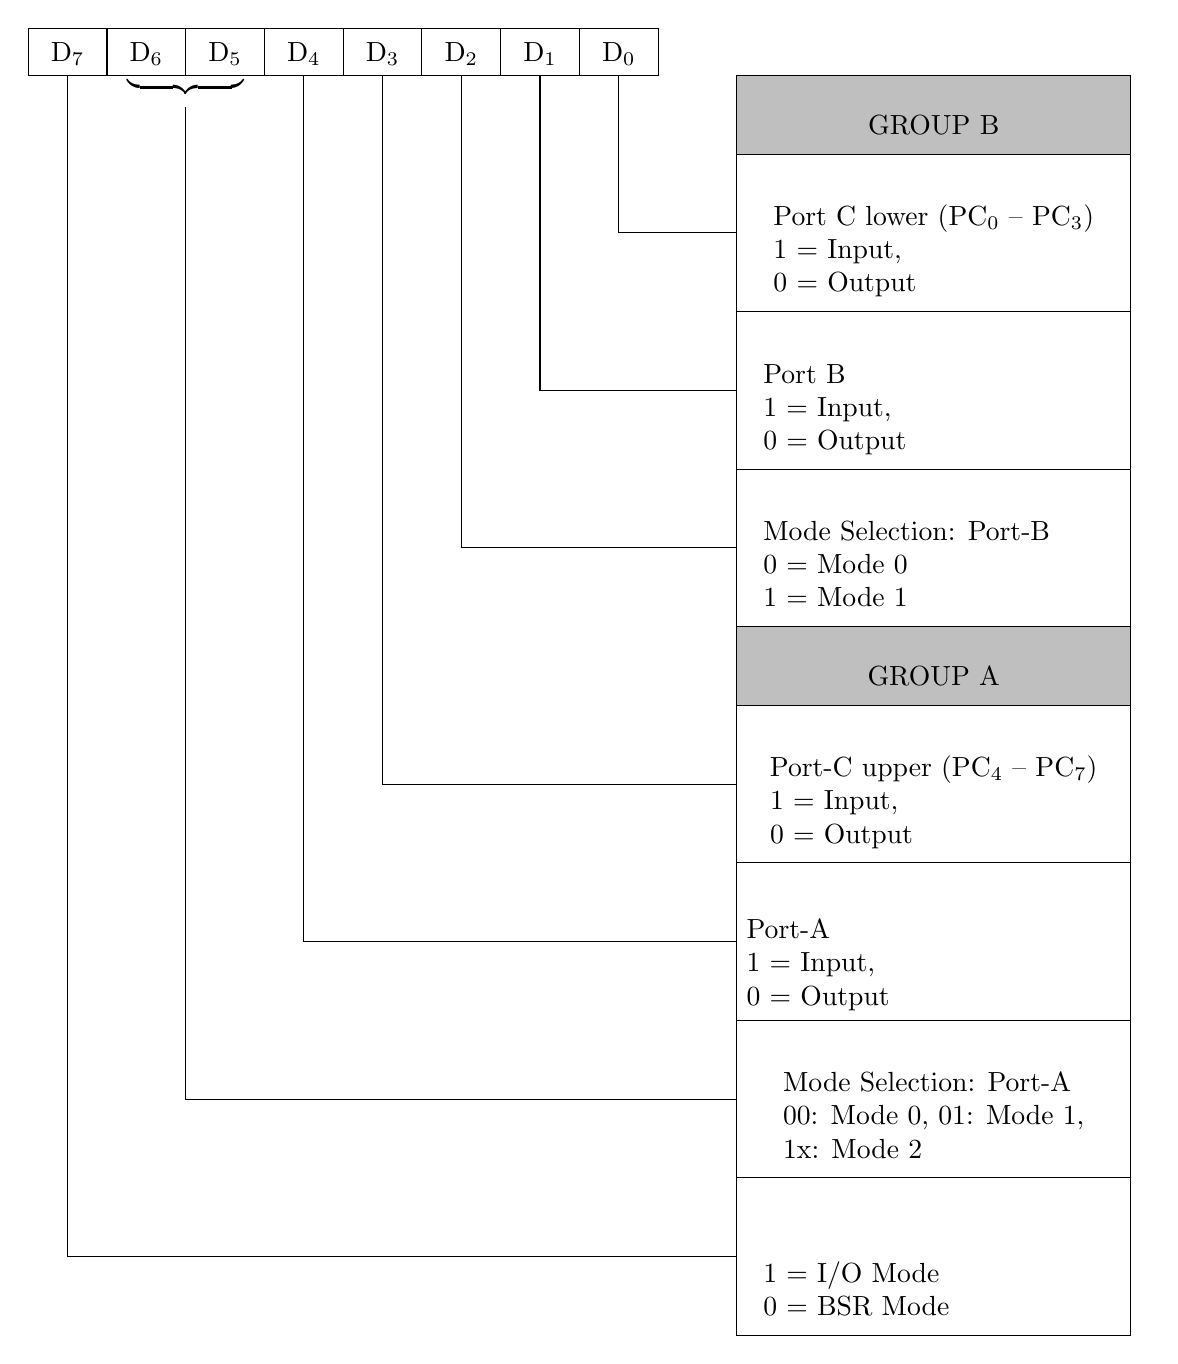
\begin{tikzpicture}
  \foreach \x in {1,...,8}
  {
    \FPeval{\lbl}{clip(8-\x)}
    \draw (\x,16) rectangle (\x+1,16.6) ;
    \draw (\x+0.5,16) node[anchor=south] {D$_{\lbl}$} ;
  }
  \foreach \y in {0,2,4,6}
  {
    \draw (10,\y) rectangle (15,\y+2) ;
  }
  \draw[fill=gray!50!white] (10,8) rectangle (15,9) ;
  \foreach \y in {9,11,13}
  {
    \draw (10,\y) rectangle (15,\y+2) ;
  }
  \draw[fill=gray!50!white] (10,15) rectangle (15,16) ;
  \draw (10,0) node[above right] {
    \begin{tabular}{l}
      1 = I/O Mode \\
      0 = BSR Mode
    \end{tabular}

  } ;
  \draw (12.5,2) node[anchor=south] {
    \begin{tabular}{l}
      Mode Selection: Port-A \\
      00: Mode 0, 01: Mode 1, \\
      1x: Mode 2
    \end{tabular}
  } ;
  \draw (10,4) node[above right] {
    \parbox[t]{5cm}{
      Port-A \\
      1 = Input, \\
      0 = Output
    }
  } ;
  \draw (12.5,6) node[anchor=south] {
    \begin{tabular}{l}
      Port-C upper (PC$_{4}$ -- PC$_{7}$) \\
      1 = Input, \\
      0 = Output
    \end{tabular}
  } ;
  \draw (12.5,8) node[anchor=south] {
    \begin{tabular}{l}
      GROUP A
    \end{tabular}
  } ;
  \draw (10,9) node[above right] {
    \begin{tabular}{l}
      Mode Selection: Port-B \\
      0 = Mode 0\\
      1 = Mode 1
    \end{tabular}
  } ;
  \draw (10,11) node[above right] {
    \begin{tabular}{l}
      Port B \\
      1 = Input, \\
      0 = Output
    \end{tabular}
  } ;
  \draw (12.5,13) node[anchor=south] {
    \begin{tabular}{l}
      Port C lower (PC$_{0}$ -- PC$_{3}$) \\
      1 = Input, \\
      0 = Output
    \end{tabular}
  } ;
  \draw (12.5,15) node[anchor=south] {
    \begin{tabular}{l}
      GROUP B
    \end{tabular}
  } ;
  \draw (1.5,16) |- (10,1) ;
  \draw (3,15.6)node[above]{$\underbrace{\phantom{aaaaaaaa}}$} to (3,3) to  (10,3) ;
  \draw (4.5,16) |- (10,5) ;
  \draw (5.5,16) |- (10,7) ;
  \draw (6.5,16) |- (10,10) ;
  \draw (7.5,16) |- (10,12) ;
  \draw (8.5,16) |- (10,14) ;
\end{tikzpicture}

  \end{center}
  % ~ }
\end{figure}

\newpage
\subsection{The circuit diagram of Logic Controller}
\begin{figure}[h]
  \scalebox{0.9}{
    \begin{circuitikz}[scale=1]
  \draw
  (1,0)node[not port] (mynot1) {} 
  (1,2)node[not port] (mynot2) {} 
  (1,4)node[not port] (mynot3) {} 
  (1,6)node[not port] (mynot4) {} 
  (1,8)node[not port] (mynot5) {} 
  (1,10)node[not port] (mynot6) {} 
  (1,12)node[not port] (mynot7) {} 
  (1,14)node[not port] (mynot8) {} 
  (14,-1)node[not port] (mynot9) {} 
  (14,1)node[not port] (mynot10) {} 
  (14,3)node[not port] (mynot11) {} 
  (14,5)node[not port] (mynot12) {} 
  (14,7)node[not port] (mynot13) {} 
  (14,9)node[not port] (mynot14) {} 
  (14,11)node[not port] (mynot15) {} 
  (14,13)node[not port] (mynot16) {} 
  [led] (3,0) to (mynot1.out) 
  (-1,0) node[anchor=west]{PA$_{7}$}
  [R,*-] (5,0) to (3,0);
  \draw 
  [led] (3,2) to (mynot2.out) 
  (-1,2) node[anchor=west]{PA$_{6}$}
  [R,*-] (5,2) to (3,2);
  \draw 
  [led] (3,4) to (mynot3.out)
  (-1,4) node[anchor=west]{PA$_{5}$}
  [R,*-] (5,4) to (3,4); \draw
  [led] (3,6) to (mynot4.out)
  (-1,6) node[anchor=west]{PA$_{4}$}
  [R,*-] (5,6) to (3,6); \draw
  [led] (3,8) to (mynot5.out)
  (-1,8) node[anchor=west]{PA$_{3}$}
  [R,*-] (5,8) to (3,8); \draw
  [led] (3,10) to (mynot6.out)
  (-1,10) node[anchor=west]{PA$_{2}$}
  [R,*-] (5,10) to (3,10); \draw
  [led] (3,12) to (mynot7.out)
  (-1,12) node[anchor=west]{PA$_{1}$}
  [R,*-] (5,12) to (3,12); \draw
  [led] (3,14) to (mynot8.out)
  (-1,14) node[anchor=west]{PA$_{0}$}
  (0,15) node[anchor=north]{\bf Port A (Output)}
  [R,*-] (5,14) to (3,14); \draw
  (5,0) to (5,15)node[ocirc]{+5V};
  \draw 
  [closing switch] (9,-1) to (mynot9.in);
  \draw 
  [closing switch] (9,1) to (mynot10.in);
  \draw 
  [closing switch] (9,3) to (mynot11.in);
  \draw 
  [closing switch] (9,5) to (mynot12.in);
  \draw 
  [closing switch] (9,7) to (mynot13.in);
  \draw 
  [closing switch] (9,9) to (mynot14.in);
  \draw 
  [closing switch] (9,11) to (mynot15.in);
  \draw 
  [closing switch] (9,13) to (mynot16.in);
  \draw 
  (9,13) to (9,-3)node[ground]{};
  \draw 
  (5,0) to [led](10,0) to [R](12,0) -| (mynot9.in) 
  (15.5,-1) node[anchor=east]{PB$_{7}$} ;
  \draw 
  (5,2) to [led](10,2) to [R](12,2) -| (mynot10.in) 
  (15.5,1) node[anchor=east]{PB$_{6}$} ;
  \draw 
  (5,4) to [led](10,4) to [R](12,4) -| (mynot11.in) 
  (15.5,3) node[anchor=east]{PB$_{5}$} ;
  \draw 
  (5,6) to [led](10,6) to [R](12,6) -| (mynot12.in) 
  (15.5,5) node[anchor=east]{PB$_{4}$} ;
  \draw 
  (5,8) to [led](10,8) to [R](12,8) -| (mynot13.in) 
  (15.5,7) node[anchor=east]{PB$_{3}$} ;
  \draw 
  (5,10) to [led](10,10) to [R](12,10) -| (mynot14.in) 
  (15.5,9) node[anchor=east]{PB$_{2}$} ;
  \draw             
  (5,12) to [led](10,12) to [R](12,12) -| (mynot15.in) 
  (15.5,11) node[anchor=east]{PB$_{1}$} ;
  \draw             
  (5,14) to [led](10,14) to [R](12,14) -| (mynot16.in) 
  (15.5,13) node[anchor=east]{PB$_{0}$} 
  (15,15) node[anchor=north]{\bf Port B\newline (Input)} ;
\end{circuitikz}

  }
\end{figure}

\newpage
\subsection{The circuit diagram of Display Interface}
\begin{figure}[H]
  \scalebox{0.5}{
    \begin{circuitikz}[scale=1]
  \coordinate(A) at (\x+2.25,3);
  \draw (\x,0) rectangle (\x+4.5,5) ;
  \begin{scope}[xslant=0.1]
    \SSGNb{A}{}
  \end{scope}
  \foreach \h in {1,...,8}
  {
    \FPeval{\k}{clip(\h/2)}
    \draw (\x+\k,0) to [R](\x+\k,-2) ;
  }
  \draw (\x,-1) node[left] {330$\Omega$} ;
  \foreach \k/\lbl in {0.5/a,1/b,1.5/c,2/d,2.5/e,3/f,3.5/g,4/h}    
  {
    \draw (\x+\k,0) node[above] {\lbl} ;
  }
  \draw (\x+2,5) node[below] {Anode} ;
  \draw (\x+4.5,3) node[left] {D3} ;
  \draw (\x,3) node[left] {MAN 72} ;
  \draw (\x+2.25,5) node[above left] {14} ;
  \draw (\x+2.25,5) to (\x+2.25,6) ;
  \draw (\x,-2) rectangle (\x+4.5,-5) ;
  \foreach \k/\lbl in {0.5/A,1/B,1.5/C,2/D,2.5/E,3/F,3.5/G,4/H}    
  {
    \draw (\x+\k,-2) node[below] {\lbl} ;
  }
  \foreach \k/\lbl in {0.5/1,1/13,1.5/10,2/8,2.5/7,3/2,3.5/11,4/6}    
  {
    \draw (\x+\k+0.1,0.1) node[below left] {\scriptsize \lbl} ;
  }
  \foreach \k/\lbl in {0.5/3,1/4,1.5/5,2/6,2.5/10,3/11,3.5/12,4/13}    
  {
    \draw (\x+\k,-2.1) node[above left] {\scriptsize \lbl} ;
  }
  \draw (\x,-3) node[right] {DA} ;
  \draw (\x,-3) node[above left] {1} ;
  \draw (\x-1,-3) to (\x,-3) ;
  \draw (\x+4,-1.8) node[circ] {} to (\x+5,-1.8) to (\x+5,-3) to (\x+6,-3);
  \draw (\x,-4) node[right] {DB} ;
  \draw (\x+1,-5) node[above] {CP} ;
  \draw (\x+2.2,-5) node[above] {CL} ;
  \draw (\x+3.4,-5) node[above] {VCC} ;
  \draw (\x+1,-5) to (\x+1,-10) ;
  \draw (\x+2.2,-5) to (\x+2.2,-6) node[circ] {};
  \draw (\x+3.4,-5) to (\x+3.4,-6) node[circ] {} ;
  \draw (\x+3.4,-6) to [C](\x+3.4,-9) ;
  \draw (\x+3.4,-7) node[left] {20nF} ;
  \draw (\x+3.4,-9) node[ground] {} ;
  \draw (\x,-4) to (\x-1,-4) to (\x-1,-6) to (\x+6,-6) node[circ] {} ;
  \draw (\x+4.5,-3.5) -| (\x+5.5,-4.5) node[ground] {} ;
  \draw (\x+4.5,-3.5) node[above right] {7} ;

  \renewcommand{\x}{7}

  \coordinate(A) at (\x+2.25,3);
  \draw (\x,0) rectangle (\x+4.5,5) ;
  \begin{scope}[xslant=0.1]
    \SSGNb{A}{}
  \end{scope}
  \foreach \h in {1,...,8}
  {
    \FPeval{\k}{clip(\h/2)}
    \draw (\x+\k,0) to [R](\x+\k,-2) ;
  }
  \draw (\x,-1) node[left] {330$\Omega$} ;
  \foreach \k/\lbl in {0.5/a,1/b,1.5/c,2/d,2.5/e,3/f,3.5/g,4/h}    
  {
    \draw (\x+\k,0) node[above] {\lbl} ;
  }
  \draw (\x+2,5) node[below] {Anode} ;
  \draw (\x+4.5,3) node[left] {D3} ;
  \draw (\x,3) node[left] {MAN 72} ;
  \draw (\x+2.25,5) node[above left] {14} ;
  \draw (\x+2.25,5) to (\x+2.25,6) ;
  \draw (\x,-2) rectangle (\x+4.5,-5) ;
  \foreach \k/\lbl in {0.5/A,1/B,1.5/C,2/D,2.5/E,3/F,3.5/G,4/H}    
  {
    \draw (\x+\k,-2) node[below] {\lbl} ;
  }
  \foreach \k/\lbl in {0.5/1,1/13,1.5/10,2/8,2.5/7,3/2,3.5/11,4/6}    
  {
    \draw (\x+\k+0.1,0.1) node[below left] {\scriptsize \lbl} ;
  }
  \foreach \k/\lbl in {0.5/3,1/4,1.5/5,2/6,2.5/10,3/11,3.5/12,4/13}    
  {
    \draw (\x+\k,-2.1) node[above left] {\scriptsize \lbl} ;
  }
  \draw (\x,-3) node[right] {DA} ;
  \draw (\x,-3) node[above left] {1} ;
  \draw (\x-1,-3) to (\x,-3) ;
  \draw (\x+4,-1.8) node[circ] {} to (\x+5,-1.8) to (\x+5,-3) to (\x+6,-3);
  \draw (\x,-4) node[right] {DB} ;
  \draw (\x+1,-5) node[above] {CP} ;
  \draw (\x+2.2,-5) node[above] {CL} ;
  \draw (\x+3.4,-5) node[above] {VCC} ;
  \draw (\x+1,-5) to (\x+1,-10) ;
  \draw (\x+2.2,-5) to (\x+2.2,-6) node[circ] {};
  \draw (\x+3.4,-5) to (\x+3.4,-6) node[circ] {} ;
  \draw (\x+3.4,-6) to [C](\x+3.4,-9) ;
  \draw (\x+3.4,-7) node[left] {20nF} ;
  \draw (\x+3.4,-9) node[ground] {} ;
  \draw (\x,-4) to (\x-1,-4) to (\x-1,-6) to (\x+6,-6) node[circ] {} ;
  \draw (\x+4.5,-3.5) -| (\x+5.5,-4.5) node[ground] {} ;
  \draw (\x+4.5,-3.5) node[above right] {7} ;

  \renewcommand{\x}{14}

  \coordinate(A) at (\x+2.25,3);
  \draw (\x,0) rectangle (\x+4.5,5) ;
  \begin{scope}[xslant=0.1]
    \SSGNb{A}{}
  \end{scope}
  \foreach \h in {1,...,8}
  {
    \FPeval{\k}{clip(\h/2)}
    \draw (\x+\k,0) to [R](\x+\k,-2) ;
  }
  \draw (\x,-1) node[left] {330$\Omega$} ;
  \foreach \k/\lbl in {0.5/a,1/b,1.5/c,2/d,2.5/e,3/f,3.5/g,4/h}    
  {
    \draw (\x+\k,0) node[above] {\lbl} ;
  }
  \draw (\x+2,5) node[below] {Anode} ;
  \draw (\x+4.5,3) node[left] {D3} ;
  \draw (\x,3) node[left] {MAN 72} ;
  \draw (\x+2.25,5) node[above left] {14} ;
  \draw (\x+2.25,5) to (\x+2.25,6) ;
  \draw (\x,-2) rectangle (\x+4.5,-5) ;
  \foreach \k/\lbl in {0.5/A,1/B,1.5/C,2/D,2.5/E,3/F,3.5/G,4/H}    
  {
    \draw (\x+\k,-2) node[below] {\lbl} ;
  }
  \foreach \k/\lbl in {0.5/1,1/13,1.5/10,2/8,2.5/7,3/2,3.5/11,4/6}    
  {
    \draw (\x+\k+0.1,0.1) node[below left] {\scriptsize \lbl} ;
  }
  \foreach \k/\lbl in {0.5/3,1/4,1.5/5,2/6,2.5/10,3/11,3.5/12,4/13}    
  {
    \draw (\x+\k,-2.1) node[above left] {\scriptsize \lbl} ;
  }
  \draw (\x,-3) node[right] {DA} ;
  \draw (\x,-3) node[above left] {1} ;
  \draw (\x-1,-3) to (\x,-3) ;
  \draw (\x+4,-1.8) node[circ] {} to (\x+5,-1.8) to (\x+5,-3) to (\x+6,-3);
  \draw (\x,-4) node[right] {DB} ;
  \draw (\x+1,-5) node[above] {CP} ;
  \draw (\x+2.2,-5) node[above] {CL} ;
  \draw (\x+3.4,-5) node[above] {VCC} ;
  \draw (\x+1,-5) to (\x+1,-10) ;
  \draw (\x+2.2,-5) to (\x+2.2,-6) node[circ] {};
  \draw (\x+3.4,-5) to (\x+3.4,-6) node[circ] {} ;
  \draw (\x+3.4,-6) to [C](\x+3.4,-9) ;
  \draw (\x+3.4,-7) node[left] {20nF} ;
  \draw (\x+3.4,-9) node[ground] {} ;
  \draw (\x,-4) to (\x-1,-4) to (\x-1,-6) to (\x+6,-6) node[circ] {} ;
  \draw (\x+4.5,-3.5) -| (\x+5.5,-4.5) node[ground] {} ;
  \draw (\x+4.5,-3.5) node[above right] {7} ;

  \renewcommand{\x}{21}

  \coordinate(A) at (\x+2.25,3);
  \draw (\x,0) rectangle (\x+4.5,5) ;
  \begin{scope}[xslant=0.1]
    \SSGNb{A}{}
  \end{scope}
  \foreach \h in {1,...,8}
  {
    \FPeval{\k}{clip(\h/2)}
    \draw (\x+\k,0) to [R](\x+\k,-2) ;
  }
  \draw (\x,-1) node[left] {330$\Omega$} ;
  \foreach \k/\lbl in {0.5/a,1/b,1.5/c,2/d,2.5/e,3/f,3.5/g,4/h}    
  {
    \draw (\x+\k,0) node[above] {\lbl} ;
  }
  \draw (\x+2,5) node[below] {Anode} ;
  \draw (\x+4.5,3) node[left] {D3} ;
  \draw (\x,3) node[left] {MAN 72} ;
  \draw (\x+2.25,5) node[above left] {14} ;
  \draw (\x+2.25,5) to (\x+2.25,6) ;
  \draw (\x,-2) rectangle (\x+4.5,-5) ;
  \foreach \k/\lbl in {0.5/A,1/B,1.5/C,2/D,2.5/E,3/F,3.5/G,4/H}    
  {
    \draw (\x+\k,-2) node[below] {\lbl} ;
  }
  \foreach \k/\lbl in {0.5/1,1/13,1.5/10,2/8,2.5/7,3/2,3.5/11,4/6}    
  {
    \draw (\x+\k+0.1,0.1) node[below left] {\scriptsize \lbl} ;
  }
  \foreach \k/\lbl in {0.5/3,1/4,1.5/5,2/6,2.5/10,3/11,3.5/12,4/13}    
  {
    \draw (\x+\k,-2.1) node[above left] {\scriptsize \lbl} ;
  }
  \draw (\x,-3) node[right] {DA} ;
  \draw (\x,-3) node[above left] {1} ;
  \draw (\x-1,-3) to (\x,-3) ;
  \draw (\x+4,-1.8) node[circ] {} to (\x+5,-1.8) to (\x+5,-3) to (\x+6,-3);
  \draw (\x,-4) node[right] {DB} ;
  \draw (\x+1,-5) node[above] {CP} ;
  \draw (\x+2.2,-5) node[above] {CL} ;
  \draw (\x+3.4,-5) node[above] {VCC} ;
  \draw (\x+1,-5) to (\x+1,-10) ;
  \draw (\x+2.2,-5) to (\x+2.2,-6) node[circ] {};
  \draw (\x+3.4,-5) to (\x+3.4,-6) node[circ] {} ;
  \draw (\x+3.4,-6) to [C](\x+3.4,-9) ;
  \draw (\x+3.4,-7) node[left] {20nF} ;
  \draw (\x+3.4,-9) node[ground] {} ;
  \draw (\x,-4) to (\x-1,-4) to (\x-1,-6) to (\x+6,-6) node[circ] {} ;
  \draw (\x+4.5,-3.5) -| (\x+5.5,-4.5) node[ground] {} ;
  \draw (\x+4.5,-3.5) node[above right] {7} ;



  \draw (\x+6,-6) to (\x+6,-8)node[ocirc] {} ;
  \draw (\x+6,-8)node[below] {+5V} ;
  \draw (\x+6,-6) to (\x+6,6) to (\x-18.75,6) ;
  \draw (\x+1,-10) to (\x-20,-10) ;
  \draw (1,-10) to (1,-11) ;
  \draw (2,-11)node[not port,rotate=180] (n1) {} ;
  \draw (1.7,-11)node[above left] {10} ;
  \draw (2.5,-11)node[above right] {11} ;
  \draw (2.2,-11)node[] {U5} ;
  \draw (5,-11)node[not port,rotate=180] (n2) {} ;
  \draw (4.7,-11)node[above left] {12} ;
  \draw (5.5,-11)node[above right] {13} ;
  \draw (5.2,-11)node[] {U5} ;
  \draw (3,-11) to (n1.in) ;
  \draw (n2.out) to (n1.in) ;
  \draw (n1.out) to (1,-11);
  \draw (-1,-3) to (-2,-3) to (-2,-14) ;
  \draw (2,-14)node[not port,rotate=180] (n3) {} ;
  \draw (1.7,-14)node[above left] {6} ;
  \draw (2.5,-14)node[above right] {5} ;
  \draw (2.2,-14)node[] {U5} ;
  \draw (5,-14)node[not port,rotate=180] (n4) {} ;
  \draw (4.7,-14)node[above left] {4} ;
  \draw (5.5,-14)node[above right] {3} ;
  \draw (5.2,-14)node[] {U5} ;
  \draw (4.2,-15)node[] {74LS04} ;
  \draw (n4.out) to (n3.in) ;
  \draw (n3.out) to (-2,-14);
  \draw (10.5,-15) |- (n4.in) ;
  \draw (13.5,-15) |- (n2.in) ;
  \foreach \h/\lb/\lbl in {10/13/PB0,11/25/VCC,12/26/GND,13/5/PC0}
  {
    \draw (\h,-15) rectangle (\h+1,-16) ;
    \draw (\h+0.5,-16) node[above] {\lb} ;
    \draw (\h+0.5,-16) node[below] {\scriptsize \lbl} ;
  }
\end{circuitikz}

  }
\end{figure}
\begin{figure}[H]
  \scalebox{0.6}{
    \renewcommand{\x}{0}
\begin{circuitikz}[scale=1]
  \foreach \h/\bn/\hn in {0/11000000/F0,1/11111001/F9,2/10100100/A4,3/10110000/B0, 4/10011001/99, 5/10010010/92, 6/10000010/82, 7/11111000/F8}
  {
    \coordinate(A) at (\x+2.25+3*\h,3);
    \begin{scope}[xslant=0.1]
      \SSGNb{A}{\h}
    \end{scope}
    \draw (\x+2.25+3*\h,1) node[below] {\bn} ;
    \draw (\x+2.25+3*\h,0) node[below] {\hn} ;
  }
  \foreach \h/\bn/\hn in {8/10000000/80,9/10011000/98,10/10001000/88,11/10000011/83,12/11000100/C6,13/10100001/A1,14/10000100/86,15/10001110/8E}
  {
    \FPeval{\res}{clip(\h-8)} ;
    \coordinate(A) at (\x+2.25+3*\res,-2);
    \begin{scope}[xslant=0.1]
      \SSGNb{A}{\h}
    \end{scope}
    \draw (\x+2.25+3*\res,-4) node[below] {\bn} ;
    \draw (\x+2.25+3*\res,-5) node[below] {\hn} ;
  }
  \coordinate(B) at (2.25,6);
  \SSGLeg{B}
  \draw (5.25,6) node[] {SSC: hgfedcba} ;
\end{circuitikz}

  }
\end{figure}

\newpage
\subsection{Keyboard Interface}
\begin{figure}[H]
  \scalebox{0.9}{
    \begin{circuitikz}[scale=1]
  \foreach \x/\y in {0/1,0/3,0/5}
  {\draw
    (\x,\y)node[circ]{} to (\x+0.33,\y+0.33)
    (\x+0.66,\y+0.66) to (\x+1,\y+1) node[circ]{}
    (\x+0.21313,\y+0.354546) to (\x+0.64545,\y+0.786875) 
    (\x+0.429289,\y+0.57071) to (\x+0.14644661,\y+0.85355339) ;
  }
  \foreach \x/\y in {2/1,2/3,2/5}
  {\draw
    (\x,\y)node[circ]{} to (\x+0.33,\y+0.33)
    (\x+0.66,\y+0.66) to (\x+1,\y+1) node[circ]{}
    (\x+0.21313,\y+0.354546) to (\x+0.64545,\y+0.786875) 
    (\x+0.429289,\y+0.57071) to (\x+0.14644661,\y+0.85355339) ;
  }
  \foreach \x/\y in {4/1,4/3,4/5}
  {\draw
    (\x,\y)node[circ]{} to (\x+0.33,\y+0.33)
    (\x+0.66,\y+0.66) to (\x+1,\y+1) node[circ]{}
    (\x+0.21313,\y+0.354546) to (\x+0.64545,\y+0.786875) 
    (\x+0.429289,\y+0.57071) to (\x+0.14644661,\y+0.85355339) ;
  }
  \foreach \x/\y in {6/1,6/3,6/5}
  {\draw
    (\x,\y)node[circ]{} to (\x+0.33,\y+0.33)
    (\x+0.66,\y+0.66) to (\x+1,\y+1) node[circ]{}
    (\x+0.21313,\y+0.354546) to (\x+0.64545,\y+0.786875) 
    (\x+0.429289,\y+0.57071) to (\x+0.14644661,\y+0.85355339) ;
  }
  \foreach \x/\y in {8/1,8/3,8/5}
  {\draw
    (\x,\y)node[circ]{} to (\x+0.33,\y+0.33)
    (\x+0.66,\y+0.66) to (\x+1,\y+1) node[circ]{}
    (\x+0.21313,\y+0.354546) to (\x+0.64545,\y+0.786875) 
    (\x+0.429289,\y+0.57071) to (\x+0.14644661,\y+0.85355339) ;
  }
  \foreach \x/\y in {10/1,10/3,10/5}
  {\draw
    (\x,\y)node[circ]{} to (\x+0.33,\y+0.33)
    (\x+0.66,\y+0.66) to (\x+1,\y+1) node[circ]{}
    (\x+0.21313,\y+0.354546) to (\x+0.64545,\y+0.786875) 
    (\x+0.429289,\y+0.57071) to (\x+0.14644661,\y+0.85355339) ;
  }
  \foreach \x/\y in {12/1,12/3,12/5}
  {\draw
    (\x,\y)node[circ]{} to (\x+0.33,\y+0.33)
    (\x+0.66,\y+0.66) to (\x+1,\y+1) node[circ]{}
    (\x+0.21313,\y+0.354546) to (\x+0.64545,\y+0.786875) 
    (\x+0.429289,\y+0.57071) to (\x+0.14644661,\y+0.85355339) ;
  }
  \foreach \x/\y in {14/1,14/3,14/5}
  {\draw
    (\x,\y)node[circ]{} to (\x+0.33,\y+0.33)
    (\x+0.66,\y+0.66) to (\x+1,\y+1) node[circ]{}
    (\x+0.21313,\y+0.354546) to (\x+0.64545,\y+0.786875) 
    (\x+0.429289,\y+0.57071) to (\x+0.14644661,\y+0.85355339) ;
  }
  \foreach \y in {1,3,5}
  {
    \draw (-1,\y) to (16,\y) ;
  }
  \foreach \x in {1,3,5,7,9,11,13,15}
  {\draw
    (\x,-4) to (\x,7) ;
  }
  \foreach \x in {1,3,5,7,9,11,13,15}
  {
    \draw [R](\x-1,0) to (\x-1,-3)node[ground]{}  ;
    \draw (\x-1,0) to (\x,0)node[circ]{};
  }
  \draw (0,6.5) node[anchor=north]{AC} ;
  \draw (2,6.5) node[anchor=north]{CE} ;
  \draw (4,6.5) node[anchor=north]{CHK} ;
  \draw (6,6.5) node[anchor=north]{=} ;
  \draw (8,6.5) node[anchor=north]{MC} ;
  \draw (10,6.5) node[anchor=north]{MR} ;
  \draw (12,6.5) node[anchor=north]{M} ;
  \draw (14,6.5) node[anchor=north]{M+} ;
  \draw (0,4.5) node[anchor=north]{8} ;
  \draw (2,4.5) node[anchor=north]{9} ;
  \draw (4,4.5) node[anchor=north]{$\cdot$} ;
  \draw (6,4.5) node[anchor=north]{+} ;
  \draw (8,4.5) node[anchor=north]{$-$} ;
  \draw (10,4.5) node[anchor=north]{$\times$} ;
  \draw (12,4.5) node[anchor=north]{/} ;
  \draw (14,4.5) node[anchor=north]{\%} ;
  \draw (0,2.5) node[anchor=north]{0} ;
  \draw (2,2.5) node[anchor=north]{1} ;
  \draw (4,2.5) node[anchor=north]{2} ;
  \draw (6,2.5) node[anchor=north]{3} ;
  \draw (8,2.5) node[anchor=north]{4} ;
  \draw (10,2.5) node[anchor=north]{5} ;
  \draw (12,2.5) node[anchor=north]{6} ;
  \draw (14,2.5) node[anchor=north]{7} ;
  \draw (1,-4) node[anchor=north]{PA$_0$} ;
  \draw (3,-4) node[anchor=north]{PA$_1$} ;
  \draw (5,-4) node[anchor=north]{PA$_2$} ;
  \draw (7,-4) node[anchor=north]{PA$_3$} ;
  \draw (9,-4) node[anchor=north]{PA$_4$} ;
  \draw (11,-4) node[anchor=north]{PA$_5$} ;
  \draw (13,-4) node[anchor=north]{PA$_6$} ;
  \draw (15,-4) node[anchor=north]{PA$_7$} ;
  \draw (16.5,7) node[anchor=north]{\bf Port-C} ;
  \draw (16.5,6.5) node[anchor=north]{\bf (output)} ;
  \draw (16,1) node[anchor=west]{PC$_0$} ;
  \draw (16,3) node[anchor=west]{PC$_1$} ;
  \draw (16,5) node[anchor=west]{PC$_2$} ;
\end{circuitikz}

  }
\end{figure}

\newpage
\subsection{The circuit diagram of DAC Interface}
\begin{figure}[H]
  \scalebox{0.7}{
    \begin{circuitikz}[scale=1]
  \draw (0,0) to (10,0) to (12,2) to (10,4) to (0,4) to (0,0);
  \draw (0,2) -| (-3,0) to [R](-3,-2) ;
  \draw[->] (-3,-2) -- (-3,-3);
  \draw (0,1) -| (-2,0) to [R](-2,-2) ;
  \draw (-2,-2) -- (-2,-3)node[ground]{};
  \draw[->] (2,0) -- (2,-2) ;
  \draw (2,-1) to (1,-1) to [C](1,-2) to (1,-3)node[ground]{};
  \draw[->] (4,0) to (4,-2) ;
  \draw (7,0) to (7,-1) to [C](4,-1) to (3,-1) to [C](3,-2) to (3,-3)node[ground]{} ;
  \draw (9,0) to (9,-3)node[ground]{};
  \draw (14,1) -- (14,3) -- (16,2) -- (14,1) ;
  \draw (11.5,2.5) -- (14,2.5) ;
  \draw (14,1.5) to (13,1.5) to [R](13,-2) to (13,-3)node[ground]{} ;
  \draw (16,2) -- (18,2) node[ocirc]{} ;
  \draw (13,2.5) to (13,3.5) to [R](16.5,3.5) to (16.5,2) ;
  \draw (14.5,1.25) to (14.5,0.5) to [R](16,0.5) to (16,2) ;
  \draw (2,-2)   node[anchor=north]{$+12$V} ;
  \draw (4,-2)   node[anchor=north]{$-12$V} ;
  \draw (3,-1)   node[anchor=south]{$0.1\mu$F} ;
  \draw (1,-1)   node[anchor=south]{$0.1\mu$F} ;
  \draw (-1.8,-1)   node[anchor=west]{$3.3$K} ;
  \draw (-3.2,-1)   node[anchor=east]{$3.3$K} ;
  \draw (-3,-3)   node[anchor=north]{V$_{\mathrm{REF}}$} ;
  \draw (-3,-3.5)   node[anchor=north]{(10V)} ;
  \draw (15,3.8)   node[anchor=south]{2K} ;
  \draw (15,0.8)   node[anchor=south]{10K} ;
  \draw (12.8,0)   node[anchor=east]{2K} ;
  \draw (14,2.5)   node[anchor=west]{$+$} ;
  \draw (14,1.5)   node[anchor=west]{$-$} ;
  \foreach \lbl/\x in {5/1,6/2,7/3,8/4,9/5,10/6,11/7,12/8}
  {
    \FPeval{\tmp}{clip(8-\x)}
    \draw (\x,4)   node[anchor=north]{\lbl} ;
    \draw (\x+0.5,4)   node[anchor=south]{\tmp} ;
  }
  \draw (0,2)   node[anchor=west]{14} ;
  \draw (0,1)   node[anchor=west]{15} ;
  \draw (2,0)   node[anchor=south]{13} ;
  \draw (4,0)   node[anchor=south]{3} ;
  \draw (7,0)   node[anchor=south]{16} ;
  \draw (9,0)   node[anchor=south]{2} ;
  \foreach \x in {1,2,3,4,5,6,7,8}
  {
    \draw (\x-0.5,5) rectangle (\x+0.5,6) ;
    \draw (\x,5) to (\x,4) ;
  }
  \draw (18.5,2)   node[anchor=north]{X$_{\mathrm{OUT}}$} ;
  \draw (19.5,1)   node[anchor=north]{\bf ANALOG OUTPUT} ;
  \draw[<->] (15.4,0) to (15.4,-1) ;
  \draw (15.4,-1)   node[anchor=north]{$-$12V} ;
  \draw (0,5.5)   node[anchor=east]{\bf Port-A} ;
  \draw (6,7)   node[anchor=east]{$\underbrace{\textrm{DIGITAL INPUT}}$} ;
  \draw (6,2)   node[anchor=east]{\bf \Large DAC 0800} ;
\end{circuitikz}

  }
\end{figure}
\begin{figure}[H]
  \scalebox{0.7}{
    \begin{circuitikz}[scale=1]
  \draw (0,0) to (10,0) to (12,2) to (10,4) to (0,4) to (0,0);
  \draw (0,2) -| (-3,0) to [R](-3,-2) ;
  \draw[->] (-3,-2) -- (-3,-3);
  \draw (0,1) -| (-2,0) to [R](-2,-2) ;
  \draw (-2,-2) -- (-2,-3)node[ground]{};
  \draw[->] (2,0) -- (2,-2) ;
  \draw (2,-1) to (1,-1) to [C](1,-2) to (1,-3)node[ground]{};
  \draw[->] (4,0) to (4,-2) ;
  \draw (7,0) to (7,-1) to [C](4,-1) to (3,-1) to [C](3,-2) to (3,-3)node[ground]{} ;
  \draw (9,0) to (9,-3)node[ground]{};
  \draw (14,1) -- (14,3) -- (16,2) -- (14,1) ;
  \draw (11.5,2.5) -- (14,2.5) ;
  \draw (14,1.5) to (13,1.5) to [R](13,-2) to (13,-3)node[ground]{} ;
  \draw (16,2) -- (18,2) node[ocirc]{} ;
  \draw (13,2.5) to (13,3.5) to [R](16.5,3.5) to (16.5,2) ;
  \draw (14.5,1.25) to (14.5,0.5) to [R](16,0.5) to (16,2) ;
  \draw (2,-2)   node[anchor=north]{$+12$V} ;
  \draw (4,-2)   node[anchor=north]{$-12$V} ;
  \draw (3,-1)   node[anchor=south]{$0.1\mu$F} ;
  \draw (1,-1)   node[anchor=south]{$0.1\mu$F} ;
  \draw (-1.8,-1)   node[anchor=west]{$3.3$K} ;
  \draw (-3.2,-1)   node[anchor=east]{$3.3$K} ;
  \draw (-3,-3)   node[anchor=north]{V$_{\mathrm{REF}}$} ;
  \draw (-3,-3.5)   node[anchor=north]{(10V)} ;
  \draw (15,3.8)   node[anchor=south]{2K} ;
  \draw (15,0.8)   node[anchor=south]{10K} ;
  \draw (12.8,0)   node[anchor=east]{2K} ;
  \draw (14,2.5)   node[anchor=west]{$+$} ;
  \draw (14,1.5)   node[anchor=west]{$-$} ;
  \foreach \lbl/\x in {5/1,6/2,7/3,8/4,9/5,10/6,11/7,12/8}
  {
    \FPeval{\tmp}{clip(8-\x)}
    \draw (\x,4)   node[anchor=north]{\lbl} ;
    \draw (\x+0.5,4)   node[anchor=south]{\tmp} ;
  }
  \draw (0,2)   node[anchor=west]{14} ;
  \draw (0,1)   node[anchor=west]{15} ;
  \draw (2,0)   node[anchor=south]{13} ;
  \draw (4,0)   node[anchor=south]{3} ;
  \draw (7,0)   node[anchor=south]{16} ;
  \draw (9,0)   node[anchor=south]{2} ;
  \foreach \x in {1,2,3,4,5,6,7,8}
  {
    \draw (\x-0.5,5) rectangle (\x+0.5,6) ;
    \draw (\x,5) to (\x,4) ;
  }
  \draw (18.5,2)   node[anchor=north]{Y$_{\mathrm{OUT}}$} ;
  \draw (19.5,1)   node[anchor=north]{\bf ANALOG OUTPUT} ;
  \draw[<->] (15.4,0) to (15.4,-1) ;
  \draw (15.4,-1)   node[anchor=north]{$-$12V} ;
  \draw (0,5.5)   node[anchor=east]{\bf Port-B} ;
  \draw (6,7)   node[anchor=east]{$\underbrace{\textrm{DIGITAL INPUT}}$} ;
  \draw (6,2)   node[anchor=east]{\bf \Large DAC 0800} ;
\end{circuitikz}

  }
\end{figure}

\newpage
\subsection{Elevator Interface}
\begin{figure}[H]
  \scalebox{0.9}{
    \begin{circuitikz}
  \draw (-4,-1) rectangle (-6,10) ;
  \foreach \y in {3,4,5,6}
  {\draw
    (-6,\y) to (-7,\y) ;
  }
  \foreach \y in {0,1,2,3,4,5,6,7,8,9}
  {\draw
    (0,\y)node[circ]{} to [D*](-2,\y) 
    (-2,\y) to [R,-o](-4,\y) ;
  }
  \foreach \y/\flreq in {0/GF,3/FF,6/SF,9/TF}
  {\draw
    (0,\y) to [D*](2,\y) 
    (2,\y) to [R](4,\y) 
    (4,\y) to (6,\y);{}
    \draw (6,\y) node[anchor=west]{\scriptsize $\overline{\mathrm{Q}}$} ;
    \draw (4,\y) node[anchor=south]{\scriptsize \flreq} ;
  }
  \foreach \y/\lbl/\flreq in {-1/PA$_{4}$/GF Request ,2/PA$_{5}$/FF Request,5/PA$_{6}$/SF Request,8/PA$_{7}$/TF Request}
  {
    \draw (6,\y) rectangle (7.2,\y+2) ;
    \draw (7.2,\y+1.5) node[ocirc]{} to (8.2,\y+1.5) node[ocirc]{} ;
    \draw (7.2,\y+1.5) node[anchor=east]{\scriptsize PR} ;
    \draw (8.7,\y+1.5) node[ocirc]{} -|  (9,\y+1.2) node[ground]{} ;
    \draw (8.2,\y+1.65) to (8.7,\y+1.65) ;
    \draw (8.45,\y+1.65) to (8.45,\y+1.85) ;
    \draw (8.45,\y+1.75) node[anchor=south]{\scriptsize \flreq} ;
    \draw (7.2,\y+0.5) node[ocirc]{} -| (9.2+\y/6,-3)  ;
    \draw (7.2,\y+.5) node[anchor=east]{\scriptsize CLR} ;
    \draw (9.2+\y/6,-3) node[anchor=north]{\scriptsize \lbl} ;
  }
  \draw (4,0)node[circ]{} to (4,-3) ;
  \draw (4.5,3)node[circ]{} to (4.5,-3) ;
  \draw (5,6)node[circ]{} to (5,-3) ;
  \draw (5.5,9)node[circ]{} to (5.5,-3) ;
  \draw (0,0) to (0,10) node[ocirc]{} ;
  \draw (0,10.5) node[anchor=north]{+5V} ;
  \draw (-7,3) node[anchor=east]{PA$_3$} ;
  \draw (-7,4) node[anchor=east]{PA$_2$} ;
  \draw (-7,5) node[anchor=east]{PA$_1$} ;
  \draw (-7,6) node[anchor=east]{PA$_0$} ;

  \draw (4,-3)   node[anchor=north]{\scriptsize PB$_3$} ;
  \draw (4.5,-3) node[anchor=north]{\scriptsize PB$_2$} ;
  \draw (5,-3)   node[anchor=north]{\scriptsize PB$_1$} ;
  \draw (5.5,-3) node[anchor=north]{\scriptsize PB$_0$} ;
  \draw (-5,5) node[anchor=north]{\large \bf 7442} ;
  \draw (-5,4) node[anchor=north]{\small DECODER} ;
  \draw (-7,2) node[anchor=north]{\bf Port-A} ;
  \draw (-7,1.5) node[anchor=north]{\bf(Out)} ;
  \draw (10,-4) node[anchor=north]{\bf Port-A} ;
  \draw (10,-4.5) node[anchor=north]{\bf(Output)} ;
  \draw (5,-4) node[anchor=north]{\bf Port-B} ;
  \draw (5,-4.5) node[anchor=north]{\bf(Input)} ;
\end{circuitikz}

  }
\end{figure}

\newpage
\subsection{The circuit diagram of Stepper Motor Driver}
\begin{figure*}[b!]
  \centering
  \begin{subfigure}[b]{0.5\textwidth}
    \scalebox{0.6}{
      \begin{circuitikz}[scale=1]
  \draw (4,0) node[npn](npn1) {} ;
  \draw (6,-1) node[npn](npn2) {} ;
  \draw (0,0) to [R](2,0) ;
  \draw (2,0)node[circ](c1){} to (npn1.base) ;
  \draw (4,3) to (10,3)node[ocirc]{};
  \draw (4,3) to [R](4,1);
  \draw (4,1) to (npn1.collector) ;
  \draw (npn1.emitter) to (4,-1) ;
  \draw (4,-1) to (npn2.base) ;
  \draw (c1) to [R](2,-2) ;
  \draw (2,-2) to (6,-2) to (npn2.emitter) ;
  \draw (6,3) to [L](npn2.collector) ;
  \draw (6,0)node[circ]{} to (10,0)node[ocirc]{} ;
  \draw (8,0)node[circ]{} to [D*](8,2.5) to (6,2.5) node[circ]{} ;
  \draw (4,-2) to (4,-3) node [ground] {} ;

  \draw (1.75,-1.25) node[anchor=east] {R$_{1}$} ;
  \draw (2.25,-1.25) node[anchor=west] {2K} ;
  \draw (1,0.25) node[anchor=south] {R$_{5}$} ;
  \draw (1,-0.25) node[anchor=north] {470E} ;
  \draw (3.75,2) node[anchor=east] {R$_{12}$} ;
  \draw (4.25,2) node[anchor=west] {620E} ;
  \draw (5.8,1.5) node[anchor=east] {C} ;
  \draw (6.2,1.5) node[anchor=west] {WDG} ;
  \draw (8.2,2) node[anchor=west] {D$_{3}$} ;
  \draw (8.2,1.5) node[anchor=west] {4001} ;
  \draw (4.2,0.5) node[anchor=west] {TR$_{3}$} ;
  \draw (4.2,0) node[anchor=west] {SL100} ;
  \draw (6.2,-1) node[anchor=west] {TR$_{6}$} ;
  \draw (6.2,-1.5) node[anchor=west] {2N3055} ;
  \draw (10,3) node[anchor=west] {$+$5/12V DC} ;
  \draw (10,0) node[anchor=west] {C} ;
  \draw (0,0) node[anchor=east] {PA$_{0}$} ;
\end{circuitikz}

    }
  \end{subfigure}%
  ~ 
  \begin{subfigure}[b]{0.5\textwidth}
    \scalebox{0.6}{
      \begin{circuitikz}[scale=1]
  \draw (4,0) node[npn](npn1) {} ;
  \draw (6,-1) node[npn](npn2) {} ;
  \draw (0,0) to [R](2,0) ;
  \draw (2,0)node[circ](c1){} to (npn1.base) ;
  \draw (4,3) to (10,3)node[ocirc]{};
  \draw (4,3) to [R](4,1);
  \draw (4,1) to (npn1.collector) ;
  \draw (npn1.emitter) to (4,-1) ;
  \draw (4,-1) to (npn2.base) ;
  \draw (c1) to [R](2,-2) ;
  \draw (2,-2) to (6,-2) to (npn2.emitter) ;
  \draw (6,3) to [L](npn2.collector) ;
  \draw (6,0)node[circ]{} to (10,0)node[ocirc]{} ;
  \draw (8,0)node[circ]{} to [D*](8,2.5) to (6,2.5) node[circ]{} ;
  \draw (4,-2) to (4,-3) node [ground] {} ;

  \draw (1.75,-1.25) node[anchor=east] {R$_{7}$} ;
  \draw (2.25,-1.25) node[anchor=west] {2K} ;
  \draw (1,0.25) node[anchor=south] {R$_{8}$} ;
  \draw (1,-0.25) node[anchor=north] {470E} ;
  \draw (3.75,2) node[anchor=east] {R$_{9}$} ;
  \draw (4.25,2) node[anchor=west] {620E} ;
  \draw (5.8,1.5) node[anchor=east] {D} ;
  \draw (6.2,1.5) node[anchor=west] {WDG} ;
  \draw (8.2,2) node[anchor=west] {D$_{4}$} ;
  \draw (8.2,1.5) node[anchor=west] {4001} ;
  \draw (4.2,0.5) node[anchor=west] {TR$_{4}$} ;
  \draw (4.2,0) node[anchor=west] {SL100} ;
  \draw (6.2,-1) node[anchor=west] {TR$_{8}$} ;
  \draw (6.2,-1.5) node[anchor=west] {2N3055} ;
  \draw (10,3) node[anchor=west] {$+$5/12V DC} ;
  \draw (10,0) node[anchor=west] {D} ;
  \draw (0,0) node[anchor=east] {PA$_{1}$} ;
\end{circuitikz}

    }
  \end{subfigure}
\end{figure*}
\begin{figure*}[b!]
  \centering
  \begin{subfigure}[b]{0.5\textwidth}
    \scalebox{0.6}{
      \begin{circuitikz}[scale=1]
  \draw (4,0) node[npn](npn1) {} ;
  \draw (6,-1) node[npn](npn2) {} ;
  \draw (0,0) to [R](2,0) ;
  \draw (2,0)node[circ](c1){} to (npn1.base) ;
  \draw (4,3) to (10,3)node[ocirc]{};
  \draw (4,3) to [R](4,1);
  \draw (4,1) to (npn1.collector) ;
  \draw (npn1.emitter) to (4,-1) ;
  \draw (4,-1) to (npn2.base) ;
  \draw (c1) to [R](2,-2) ;
  \draw (2,-2) to (6,-2) to (npn2.emitter) ;
  \draw (6,3) to [L](npn2.collector) ;
  \draw (6,0)node[circ]{} to (10,0)node[ocirc]{} ;
  \draw (8,0)node[circ]{} to [D*](8,2.5) to (6,2.5) node[circ]{} ;
  \draw (4,-2) to (4,-3) node [ground] {} ;

  \draw (1.75,-1.25) node[anchor=east] {R$_{1}$} ;
  \draw (2.25,-1.25) node[anchor=west] {2K} ;
  \draw (1,0.25) node[anchor=south] {R$_{2}$} ;
  \draw (1,-0.25) node[anchor=north] {470E} ;
  \draw (3.75,2) node[anchor=east] {R$_{10}$} ;
  \draw (4.25,2) node[anchor=west] {620E} ;
  \draw (5.8,1.5) node[anchor=east] {A} ;
  \draw (6.2,1.5) node[anchor=west] {WDG} ;
  \draw (8.2,2) node[anchor=west] {D$_{1}$} ;
  \draw (8.2,1.5) node[anchor=west] {4001} ;
  \draw (4.2,0.5) node[anchor=west] {TR$_{1}$} ;
  \draw (4.2,0) node[anchor=west] {SL100} ;
  \draw (6.2,-1) node[anchor=west] {TR$_{5}$} ;
  \draw (6.2,-1.5) node[anchor=west] {2N3055} ;
  \draw (10,3) node[anchor=west] {$+$5/12V DC} ;
  \draw (10,0) node[anchor=west] {A} ;
  \draw (0,0) node[anchor=east] {PA$_{2}$} ;
\end{circuitikz}

    }
  \end{subfigure}%
  ~ 
  \begin{subfigure}[b]{0.5\textwidth}
    \scalebox{0.6}{
      \begin{circuitikz}[scale=1]
  \draw (4,0) node[npn](npn1) {} ;
  \draw (6,-1) node[npn](npn2) {} ;
  \draw (0,0) to [R](2,0) ;
  \draw (2,0)node[circ](c1){} to (npn1.base) ;
  \draw (4,3) to (10,3)node[ocirc]{};
  \draw (4,3) to [R](4,1);
  \draw (4,1) to (npn1.collector) ;
  \draw (npn1.emitter) to (4,-1) ;
  \draw (4,-1) to (npn2.base) ;
  \draw (c1) to [R](2,-2) ;
  \draw (2,-2) to (6,-2) to (npn2.emitter) ;
  \draw (6,3) to [L](npn2.collector) ;
  \draw (6,0)node[circ]{} to (10,0)node[ocirc]{} ;
  \draw (8,0)node[circ]{} to [D*](8,2.5) to (6,2.5) node[circ]{} ;
  \draw (4,-2) to (4,-3) node [ground] {} ;

  \draw (1.75,-1.25) node[anchor=east] {R$_{3}$} ;
  \draw (2.25,-1.25) node[anchor=west] {2K} ;
  \draw (1,0.25) node[anchor=south] {R$_{4}$} ;
  \draw (1,-0.25) node[anchor=north] {470E} ;
  \draw (3.75,2) node[anchor=east] {R$_{11}$} ;
  \draw (4.25,2) node[anchor=west] {620E} ;
  \draw (5.8,1.5) node[anchor=east] {B} ;
  \draw (6.2,1.5) node[anchor=west] {WDG} ;
  \draw (8.2,2) node[anchor=west] {D$_{2}$} ;
  \draw (8.2,1.5) node[anchor=west] {4001} ;
  \draw (4.2,0.5) node[anchor=west] {TR$_{2}$} ;
  \draw (4.2,0) node[anchor=west] {SL100} ;
  \draw (6.2,-1) node[anchor=west] {TR$_{7}$} ;
  \draw (6.2,-1.5) node[anchor=west] {2N3055} ;
  \draw (10,3) node[anchor=west] {$+$5/12V DC} ;
  \draw (10,0) node[anchor=west] {B} ;
  \draw (0,0) node[anchor=east] {PA$_{3}$} ;
\end{circuitikz}

    }
  \end{subfigure}
\end{figure*}
\begin{figure*}[b!]
  \centering
  \begin{subfigure}[b]{0.3\textwidth}
    \scalebox{0.6}{
      \begin{circuitikz}[scale=1]
  \draw (0,0) rectangle (3,5) ;
  \foreach \y in {1,2,3,4} 
  {
    \FPeval{\lbl}{clip(5-\y)} 
    \draw (0,\y) to (-1,\y) ;
    \draw (0,\y) node[anchor=west] {\lbl} ;
  }
  \foreach \lbl/\y in {D/1,C/2,B/3,A/4} 
  {
    \draw (-1,\y) node[anchor=east] {\lbl} ;
  }
  \draw (1,5)node[anchor=south] {J1} ;
\end{circuitikz}

    }
  \end{subfigure}%
  ~ 
  \begin{subfigure}[b]{0.3\textwidth}
    \scalebox{0.6}{
      \begin{circuitikz}[scale=1]
  \draw (0,0) rectangle (3,4) ;
  \foreach \y in {1,2,3} 
  {
    \FPeval{\lbl}{clip(4-\y)} 
    \draw (0,\y) to (-1,\y) ;
    \draw (0,\y) node[anchor=west] {\lbl} ;
  }
  \foreach \lbl/\y in {WHT/3,BLK/2,/1} 
  {
    \draw (-1,\y) node[anchor=east] {\lbl} ;
  }
  \draw (1,4)node[anchor=south] {J3} ;
\end{circuitikz}


    }
  \end{subfigure}
  
\end{figure*}
\begin{figure*}[b!]
  \centering
  \begin{subfigure}[b]{0.3\textwidth}
    \scalebox{0.6}{
      \begin{circuitikz}[scale=1]
  \draw (0,0) rectangle (3,4) ;
  \foreach \y in {1,2,3} 
  {
    \FPeval{\lbl}{clip(4-\y)} 
    \draw (0,\y) to (-1,\y) ;
    \draw (0,\y) node[anchor=west] {\lbl} ;
  }
  \draw (0,3) to (-2,3) to (-2,-1)node[ground] {} ;
  \draw (0,2) to (-3,2) to (-3,5)node[ocirc] {} ;
  \draw (1,4)node[anchor=south] {J2} ;
  \draw (-3,5)node[anchor=south] {$+$5/12V DC} ;
\end{circuitikz}

    }
  \end{subfigure}%
  ~ 
  \begin{subfigure}[b]{0.3\textwidth}
    \scalebox{0.4}{
      \begin{circuitikz}[scale=1]
  \draw (0,0) rectangle (5,15) ;
  \foreach \n in {1,...,13}
  {
    \FPeval{\lbl}{clip(26-2*\n+2)} 
    \draw (0,\n) to (-1,\n) ;
    \draw (5,\n) to (6,\n) ;
    \draw (5,\n) node[anchor=east] {\lbl} ;
    \FPeval{\lbl}{clip(26-2*\n+1)} 
    \draw (0,\n) to (-1,\n) ;
    \draw (0,\n) to (-1,\n) ;
    \draw (0,\n) node[anchor=west] {\lbl} ;
  }
  \draw (-1,3) node[anchor=east] {PA$_{0}$} ;
  \draw (-1,4) node[anchor=east] {PA$_{2}$} ;
  \draw (6,3) node[anchor=west] {PA$_{1}$} ;
  \draw (6,4) node[anchor=west] {PA$_{3}$} ;
  \draw (2,15) node[anchor=south] {J1} ;
  \draw (2,0) node[anchor=north] {CON26A} ;
  \draw (-1,1) to (-3,1) to (-3,3)node[ocirc] {V$_{\textrm{\tiny CC}}$} ;
  \draw (6,1) to (8,1) to (8,-2)node[ground] {} ;
\end{circuitikz}

    }
  \end{subfigure}
  \begin{subfigure}[b]{0.3\textwidth}
    \scalebox{0.6}{
      \begin{circuitikz}[scale=1]
  \draw (0,0) to (8,0) node[ocirc] {} ;
  \draw (0,1) to [L](4,1) ;
  \draw [L](4,1) to (8,1)node[ocirc] {} ;
  \draw (0,0) to (0,1) ;
  \draw (4,1) to (4,2) to (8,2) node[ocirc]{} ;
  \draw (0,5) to (8,5) node[ocirc] {} ;
  \draw (0,4) to [L](4,4) ;
  \draw [L](4,4) to (8,4)node[ocirc] {} ;
  \draw (0,5) to (0,4) ;
  \draw (4,4) to (4,3) to (8,3) node[ocirc]{} ;
  \draw (2,0.75)node[anchor=north] {WDG D} ;
  \draw (6,0.75)node[anchor=north] {WDG C} ;
  \draw (6,3.75)node[anchor=north] {WDG B} ;
  \draw (2,3.75)node[anchor=north] {WDG A} ;
  \draw (8,0)node[anchor=west] {D} ;
  \draw (8,1)node[anchor=west] {C} ;
  \draw (8,2)node[anchor=west] {BLK} ;
  \draw (8,3)node[anchor=west] {WHT} ;
  \draw (8,4)node[anchor=west] {B} ;
  \draw (8,5)node[anchor=west] {A} ;
\end{circuitikz}

    }
  \end{subfigure}
\end{figure*}

\newpage
\subsection{Control Word Format}
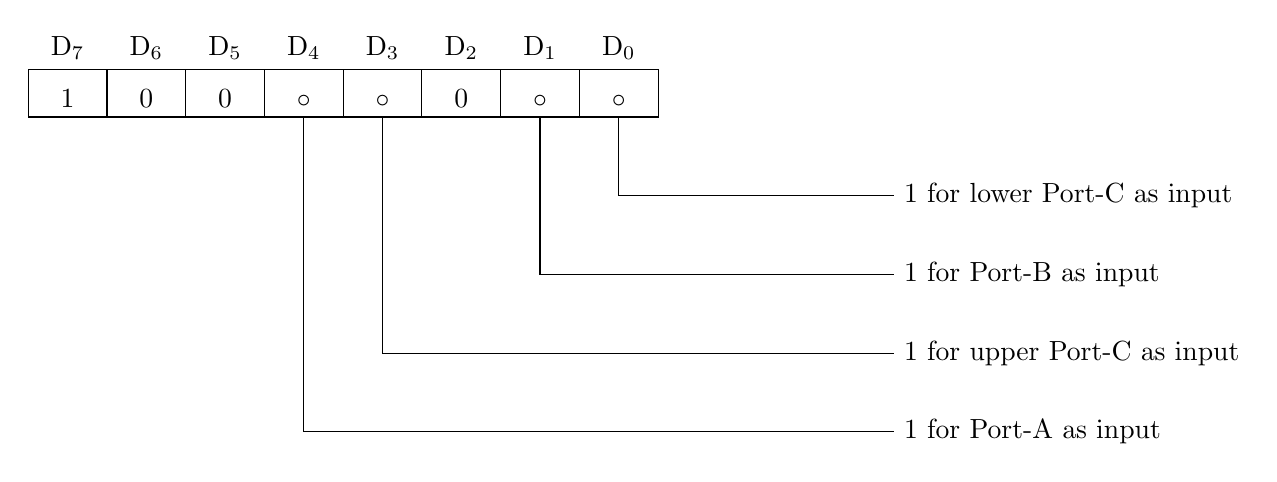
\begin{tikzpicture}
  \foreach \x/\b in {1/1,2/0,3/0,4/$\circ$,5/$\circ$, 6/0,7/$\circ$,8/$\circ$}
  {
    \FPeval{\lbl}{clip(8-\x)}
    \draw (\x,16) rectangle (\x+1,16.6) ;
    \draw (\x+0.5,16.6) node[anchor=south] {D$_{\lbl}$} ;
    \draw (\x+0.5,16) node[anchor=south] {\b} ;
  }
  \draw (4+0.5,16) |- (12,12) node[right] {1 for Port-A as input} ;
  \draw (5+0.5,16) |- (12,13) node[right] {1 for upper Port-C as input} ;
  \draw (7+0.5,16) |- (12,14) node[right] {1 for Port-B as input} ;
  \draw (8+0.5,16) |- (12,15) node[right] {1 for lower Port-C as input} ;
\end{tikzpicture}

\vspace{1cm}
\textbf{Logic controller}

CW DB 82H		; Port-A output, Port-B input; MDE-0, I/O Mode.

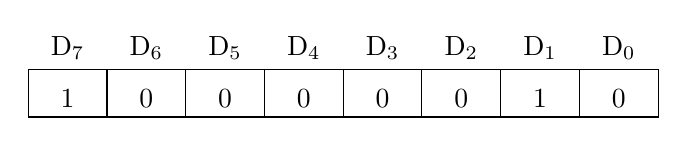
\begin{tikzpicture}
  \foreach \x/\b in {1/1,2/0,3/0,4/0,5/0, 6/0,7/1,8/0}
  {
    \FPeval{\lbl}{clip(8-\x)}
    \draw (\x,16) rectangle (\x+1,16.6) ;
    \draw (\x+0.5,16.6) node[anchor=south] {D$_{\lbl}$} ;
    \draw (\x+0.5,16) node[anchor=south] {\b} ;
  }
\end{tikzpicture}

\vspace{1cm}
\textbf{Seven Segment display}

CW DB 80H 		; Port-B output, Port-C output, Mode 0, I/O Mode

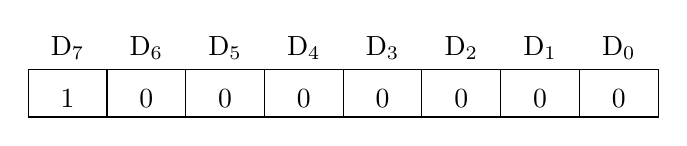
\begin{tikzpicture}
  \foreach \x/\b in {1/1,2/0,3/0,4/0,5/0, 6/0,7/0,8/0}
  {
    \FPeval{\lbl}{clip(8-\x)}
    \draw (\x,16) rectangle (\x+1,16.6) ;
    \draw (\x+0.5,16.6) node[anchor=south] {D$_{\lbl}$} ;
    \draw (\x+0.5,16) node[anchor=south] {\b} ;
  }
\end{tikzpicture}
\vspace{1cm}

\textbf{Key Board interface}

CW DB 90H   ;Port-A input, Port-C output, Mode-0, I/O Mode

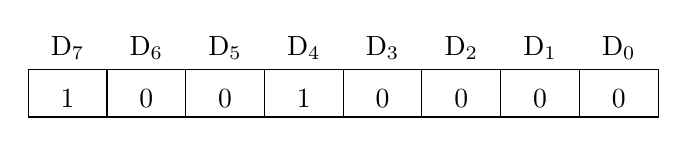
\begin{tikzpicture}
  \foreach \x/\b in {1/1,2/0,3/0,4/1,5/0, 6/0,7/0,8/0}
  {
    \FPeval{\lbl}{clip(8-\x)}
    \draw (\x,16) rectangle (\x+1,16.6) ;
    \draw (\x+0.5,16.6) node[anchor=south] {D$_{\lbl}$} ;
    \draw (\x+0.5,16) node[anchor=south] {\b} ;
  }
\end{tikzpicture}

\vspace{1cm}
\textbf{Elevator Interface}

CW DB 80H 		; Port-B output, Port-C output, Mode-0, I/O Mode

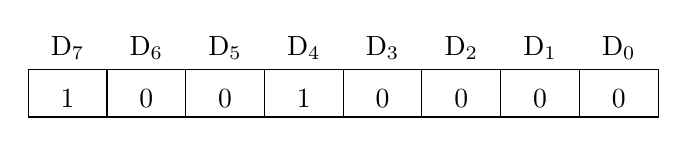
\begin{tikzpicture}
  \foreach \x/\b in {1/1,2/0,3/0,4/1,5/0, 6/0,7/0,8/0}
  {
    \FPeval{\lbl}{clip(8-\x)}
    \draw (\x,16) rectangle (\x+1,16.6) ;
    \draw (\x+0.5,16.6) node[anchor=south] {D$_{\lbl}$} ;
    \draw (\x+0.5,16) node[anchor=south] {\b} ;
  }
\end{tikzpicture}

\vspace{1cm}
\newpage
\subsection{Flag register}

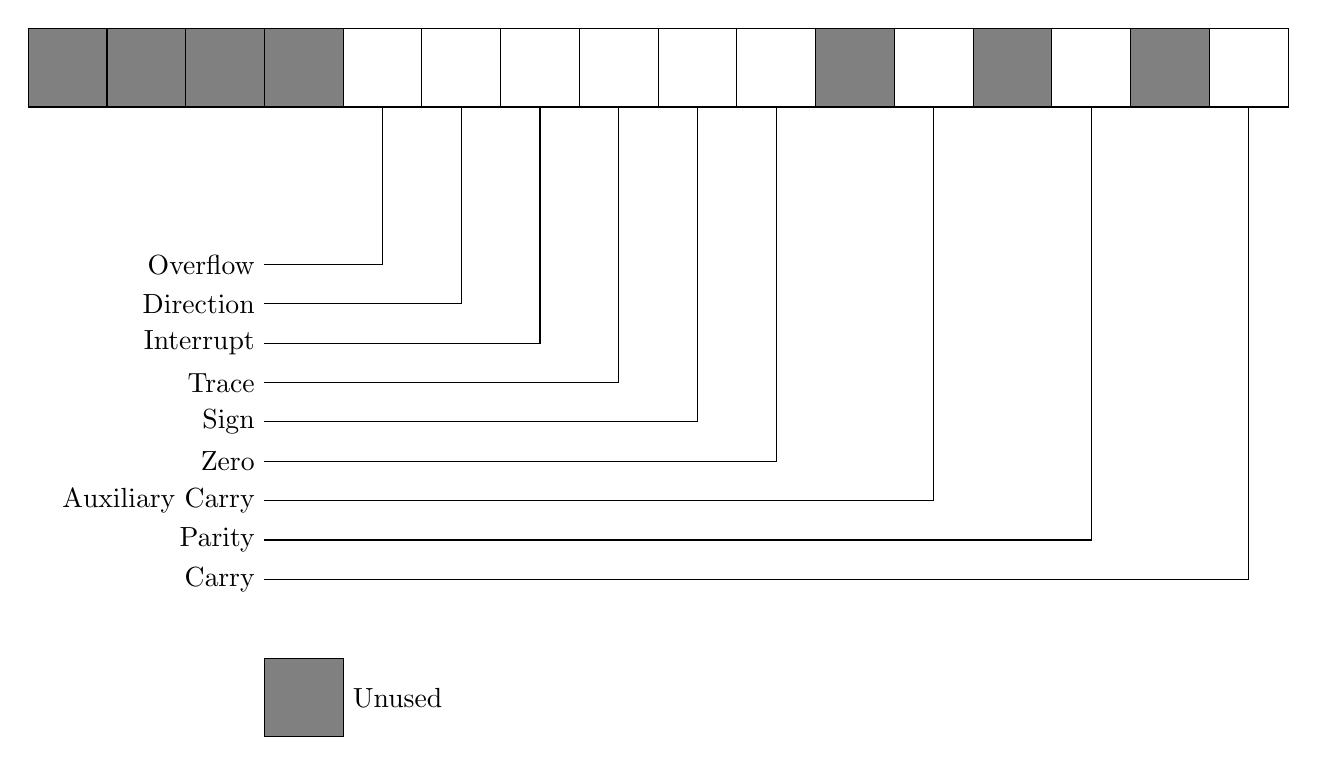
\begin{tikzpicture}
  \foreach \x/\b in {1/gray,2/gray,3/gray,4/gray,5/white, 6/white,7/white,8/white,9/white,10/white,11/gray,12/white,13/gray,14/white,15/gray,16/white}
  {
    \draw[fill=\b] (\x,16) rectangle (\x+1,17) ;
  }
  \draw (5.5,16) |- (4,14) node[left] {Overflow} ;
  \draw (6.5,16) |- (4,13.5) node[left] {Direction} ;
  \draw (7.5,16) |- (4,13) node[left] {Interrupt} ;
  \draw (8.5,16) |- (4,12.5) node[left] {Trace} ;
  \draw (9.5,16) |- (4,12) node[left] {Sign} ;
  \draw (10.5,16) |- (4,11.5) node[left] {Zero} ;
  \draw (12.5,16) |- (4,11) node[left] {Auxiliary Carry} ;
  \draw (14.5,16) |- (4,10.5) node[left] {Parity} ;
  \draw (16.5,16) |- (4,10) node[left] {Carry} ;
  \draw[fill=gray] (4,9) rectangle (5,8) ;
  \draw (5,8.5) node[right] {Unused} ;
\end{tikzpicture}

\vspace{2cm}

\begin{tabular}{ll}
  \textbf{Flag} & \textbf{Function}\\\\
  CF-Carry Flag & 
                  \parbox[t]{12cm}{ 
                  =1 if high order bit carry/borrow \\
  =0 otherwise
  } \\\\
  PF-Parity Flag & 
                   \parbox[t]{12cm}{ 
                   =1 if low order 8-bit of result contain even parity \\
  =0 otherwise
  } \\\\
  AF-Auxiliary Flag &
                      \parbox[t]{12cm}{
                      =1 if carry from/borrow to lower nibble of AL \\
  =0 otherwise
  }\\\\
  ZF-Zero Flag &
                 \parbox[t]{12cm}{
                 =1 if result is zero \\
  =0 otherwise
  } \\\\
  SF-Sign Flag &
                 \parbox[t]{12cm}{
                 =1 if MSB of result is 1 ($-$ve sign) \\
  =0 if MSB of result is 0 (+ve sign ) 
  }\\\\
  OF-Overflow Flag & 
                     \parbox[t]{12cm}{
                     =1 if result is out of range \\
  =0 otherwise 
  }
\end{tabular}

\end{document}
